\documentclass[10pt]{article}
\title{Medium Practice}
\date{15-11-2021}
\author{Aritra Roy}
\newcommand{\mathset}[1][x]{\{{#1}|0\leq{#1}\leq1\}} % defining new command for easy writing
\usepackage[margin=0.5in]{geometry}
\usepackage{amsmath, amssymb, graphicx, subcaption, float}
\graphicspath{ {./pictures/} }
\begin{document}
\maketitle
One may find the environments \textbf{bmatrix} and \textbf{pmatrix} useful for the following exercises.
\begin{flalign}
\rho_\theta=\begin{pmatrix}\cos\theta & \sin\theta\\-\sin\theta & \cos\theta \end{pmatrix}&=\begin{bmatrix}\cos\theta & \sin\theta\\-\sin\theta & \cos\theta \end{bmatrix}\\
\left[\begin{tabular}{c|c c c}
    1&0&$\cdots$&0\\
    \hline\\
    0&*&$\cdots$&*\\
    $\vdots$&$\vdots$&$\ddots$&$\vdots$\\
    0&*&$\cdots$&*
\end{tabular}\right]&=
\begin{tabular}{|c|c c c|}
    \hline
    1&0&$\cdots$&0\\
    \hline
    0&*&$\cdots$&*\\
    $\vdots$&$\vdots$&$\ddots$&$\vdots$\\
    0&*&$\cdots$&*\\
    \hline
\end{tabular}
\end{flalign}
Note the locations of the bounds on the summation in the following exercise.
\begin{flalign}
\sigma=\sqrt{\frac{1}{N}\sum_{i=1}^N p_i{(x_i-\overline{x})}^2}&=\sqrt{\frac{\displaystyle\sum_{i=1}^N p_i{(x_i-\overline{x})}^2}{N}}\\
\varphi(n)&=n\cdot\hspace{-4mm}\prod_{\begin{gathered}{p|n}\\[-1ex]{p\hspace{1mm}prime}\end{gathered}}\hspace{-4mm}\left(1-\frac{1}{p}\right)\\
{^4}{_{12}}C_2^{5+}\hspace{5mm}{^{14}}{_2}C_2^{5+}\hspace{5mm}&{{^4}{_{12}}C_2^{5+}}\hspace{5mm}{^{14}}C_2^{5+}\hspace{5mm}{_2}C_2^{5+}
\end{flalign}
In the following, the size of the /, and the spacing on the sides of | are noticable.
\begin{flalign}
\mathbb{Q}\cong\left\{\frac{a}{b}\hspace{1mm}\scalebox{2}{$|$}\hspace{1mm}a,b\in\mathbb{Z}\text{ and b}\neq0\right\} &\scalebox{2}{/}\sim\\
\frac{a}{b}\sim\frac{c}{d}\Longleftrightarrow ad-bc&=0\\
\mathset{}\\ % gives default value i.e. x
\mathset[z]  % overwriting the default value
\end{flalign}

\begin{figure}[H]
  \centering
  \begin{subfigure}[b]{0.4\linewidth}
    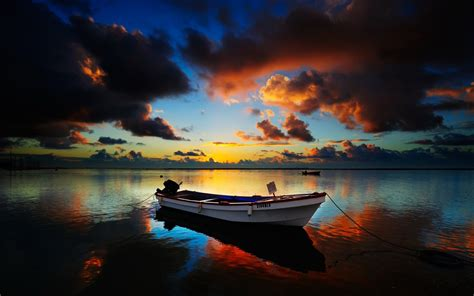
\includegraphics[width=\linewidth]{wallpaper1.jpg}
    \caption{Wallpaper 1}
  \end{subfigure}
  \begin{subfigure}[b]{0.4\linewidth}
    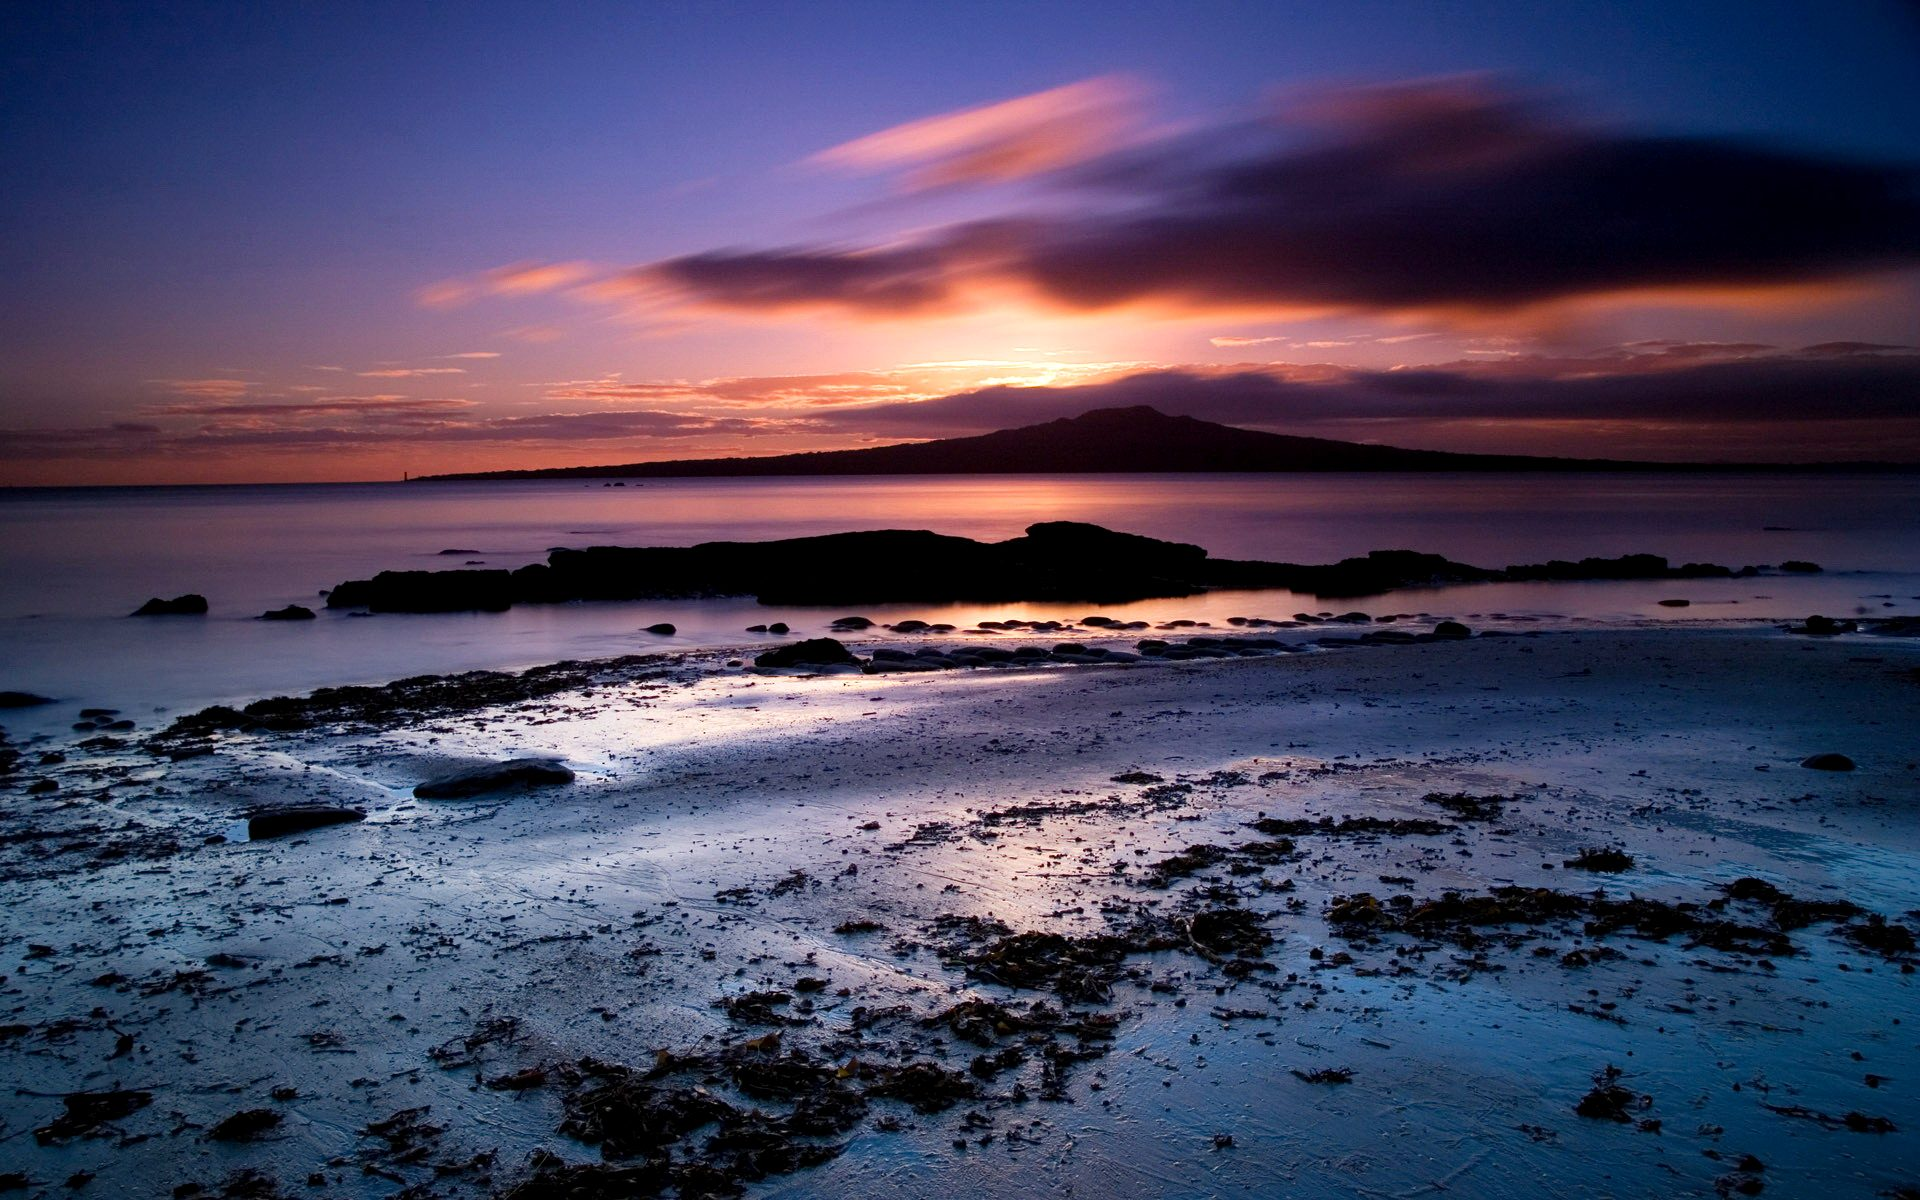
\includegraphics[width=\linewidth]{wallpaper2.jpg}
    \caption{Wallpaper 2}
  \end{subfigure}
  \caption{Image insertion}
  \label{fig:image}
\end{figure}
\end{document}